\clearpage
\subsection{Task 2: การจำแนกกลุ่มพฤติกรรมผู้เล่น (Player Segment Classification)}
\label{subsec:task2}

% ==============================================================================
% PART 1: BUSINESS CONTEXT & MACRO F1 MECHANICS
% ==============================================================================
\subsubsection{บริบททางธุรกิจและกลไกของตัวชี้วัด Macro $F_1$}
\label{subsubsec:t2_business_metric}

ในบริบทการดำเนินงานของบริษัท Karena Thailand ทีมการตลาดใช้งบประมาณส่งเสริมการขายประมาณ 60 ล้านบาทต่อเดือนสำหรับแคมเปญแบบหว่านแหครอบคลุมผู้เล่นทั้งหมด (generic campaigns) ส่งผลให้อัตราการมีส่วนร่วม (engagement rate) อยู่ในระดับต่ำมากเพียง 2--5\% ความสูญเปล่าดังกล่าวเกิดจากการส่งข้อเสนอที่ไม่สอดคล้องกับพฤติกรรมผู้เล่น เช่น การประชาสัมพันธ์ทัวร์นาเมนต์ esports ให้แก่ผู้เล่นสายผ่อนคลาย (Casual) การโฆษณาไอเทมตกแต่ง (cosmetic items) ให้แก่ผู้เล่นที่ไม่เคยเติมเงิน หรือการส่งคำเชิญกิจกรรม FiveN roleplay ไปยังผู้เล่นสายไต่อันดับอย่าง PUBE Competitive Grinder ปัญหาสำคัญเชิงโครงสร้างคือ กลุ่มผู้เล่นที่มียอดใช้จ่ายสูงสุด 5\% แรก (Whales) สร้างรายได้คิดเป็นสัดส่วนถึง 60\% ของรายได้ทั้งหมด แต่ไม่สามารถแยกแยะได้ด้วยตัวชี้วัดเชิงเดี่ยวอย่างเวลาเล่นสะสม (\feat{total\_playtime\_hours}) เนื่องจากผู้เล่นที่มีชั่วโมงเล่นสูงอาจเป็นได้ทั้งกลุ่ม Grinder ที่เน้นไต่อันดับ กลุ่ม Social ที่เน้นเล่นกับเพื่อน หรือกลุ่ม Whale ที่ลงทุนสูง การแบ่งกลุ่มพฤติกรรมผู้เล่นออกเป็น 4 กลุ่มหลัก ได้แก่ \textbf{0: Casual}, \textbf{1: Grinder}, \textbf{2: Social} และ \textbf{3: Whale} ได้อย่างแม่นยำจึงเป็นกลไกสำคัญที่ช่วยยกระดับประสิทธิผลของแคมเปญการตลาดได้ถึง 3--4 เท่า

ชุดข้อมูลของ Task 2 (ฉบับปรับปรุงใหม่วันที่ 12 พฤศจิกายน ค.ศ.~2026) ประกอบด้วยแถวฝึก (\feat{train.csv}) จำนวน 104,000 แถว และแถวทดสอบ (\feat{test.csv}) จำนวน 25,889 แถว โดยมีฟีเจอร์ตั้งต้น 44 คอลัมน์ (ไม่รวม \feat{player\_id} และคอลัมน์เป้าหมาย \feat{segment}) การกระจายตัวของคลาสในชุดฝึกมีความไม่สมดุลระดับปานกลาง คือ คลาส 0 (Casual) จำนวน 40,957 แถว (39.38\%), คลาส 1 (Grinder) จำนวน 26,032 แถว (25.03\%), คลาส 2 (Social) จำนวน 21,029 แถว (20.22\%) และคลาส 3 (Whale) จำนวน 15,982 แถว (15.37\%)

การประเมินผลใช้ตัวชี้วัด \textbf{Macro $F_1$} ซึ่งนิยามเป็นค่าเฉลี่ยเลขคณิตแบบไม่ถ่วงน้ำหนักของ $F_{1,k}$ ทั้ง 4 คลาส:
\begin{equation}
\label{eq:t2_macro_f1}
\mathrm{Macro}\ F_1 = \frac{1}{4}\sum_{k=0}^{3} F_{1,k}, \qquad
F_{1,k} = \frac{2\,\mathrm{TP}_k}{2\,\mathrm{TP}_k + \mathrm{FP}_k + \mathrm{FN}_k}
= \frac{2\,\mathbb{P}(y=k,\,\hat{y}=k)}{\pi_k + q_k}
\end{equation}
โดยที่ $\pi_k = \mathbb{P}(y=k)$ คือสัดส่วนความถี่จริง (class prior) ของคลาส $k$ และ $q_k = \mathbb{P}(\hat{y}=k)$ คือสัดส่วนการทำนายคลาส $k$ จากสมการ~(\ref{eq:t2_macro_f1}) จะเห็นกลไกทางคณิตศาสตร์ที่สำคัญสองประการ ประการแรก ทุกคลาสมีน้ำหนัก $\frac{1}{4}$ เท่ากันในเป้าหมายรวม ทำให้คลาสส่วนน้อยอย่าง Whale ($\pi_3 = 0.1537$) และ Social ($\pi_2 = 0.2022$) มีอิทธิพลต่อคะแนนรวมเท่าเทียมกับคลาส Casual ($\pi_0 = 0.3938$) ประการที่สอง ตัวหาร $\pi_k + q_k$ ของกลุ่ม Whale มีขนาดเล็กกว่ากลุ่ม Casual ราว 2.5 เท่า ดังนั้นการทายถูกหรือพลาดเพียง 1 รายการในกลุ่ม Whale จะสร้างการเปลี่ยนแปลงต่อค่า $\mathrm{Macro}\ F_1$ มากกว่ารายการในกลุ่ม Casual อย่างมีนัยสำคัญ ด้วยเหตุนี้ กฎการตัดสินใจมาตรฐาน $\hat{y}(x) = \arg\max_k P(y=k \mid x)$ ซึ่งมุ่งหาความแม่นยำรวม (0--1 loss) จึงไม่เหมาะสมที่สุดสำหรับเป้าหมาย $\mathrm{Macro}\ F_1$ เพราะมักอนุรักษนิยมต่อคลาสส่วนน้อยบริเวณรอยต่อการตัดสินใจ

% ==============================================================================
% PART 2: EDA & DATA-GENERATING STRUCTURE
% ==============================================================================
\subsubsection{ข้อค้นพบจาก EDA และโครงสร้างการสร้างข้อมูล}
\label{subsubsec:t2_eda_dgp}

การวิเคราะห์ข้อมูลเชิงลึก (EDA) ดำเนินตามกรอบการตั้งสมมติฐานและการพิสูจน์เชิงประจักษ์ (\textit{Claim $\to$ Evidence $\to$ Implication}) เพื่อค้นหาโครงสร้างที่แท้จริงของตัวสร้างข้อมูล (data-generating process)

\begin{enumerate}
  \item \textbf{การคัดกรองฟีเจอร์รบกวนบริสุทธิ์ 16 คอลัมน์ (Noise Feature Pruning):}
  \begin{itemize}
    \item \textit{Claim:} จากฟีเจอร์ดิบ 44 คอลัมน์ มีเพียง 28 คอลัมน์ที่มีสารสนเทศจำแนกพฤติกรรม (23 ฟีเจอร์ต่อเนื่อง และ 5 ฟีเจอร์ไม่ต่อเนื่อง) ส่วนอีก 16 คอลัมน์เป็นสัญญาณรบกวนบริสุทธิ์ที่ไม่ขึ้นกับคลาส
    \item \textit{Evidence:} การคำนวณ Information Gain เชิงเดี่ยวด้วย Univariate Naive Bayes พบว่าฟีเจอร์ 16 คอลัมน์ให้ค่า Information Gain $\le 0$ ทั้งหมด ได้แก่ \feat{random\_metric\_1}, \feat{random\_metric\_2}, \feat{random\_metric\_3}, \feat{region}, \feat{platform}, \feat{device\_type}, \feat{payment\_method}, \feat{language}, \feat{account\_status}, \feat{player\_type\_tag}, \feat{skill\_tier}, \feat{account\_age\_days}, \feat{preferred\_game\_mode}, \feat{avg\_match\_length}, \feat{responds\_to\_discounts} และ \feat{item\_type\_preference\_social} ในบรรดาตัวแปรเชิงหมวดหมู่ทั้งหมด มีเพียง \feat{engagement\_level} และ \feat{loyalty\_tier} ที่มีอำนาจจำแนกคลาส ส่วนตัวแปรไม่ต่อเนื่องเชิงตัวเลขอีก 3 ตัวที่คงไว้คือ \feat{competitive\_rank}, \feat{watches\_esports} และ \feat{vip\_tier}
    \item \textit{Implication:} ตัดฟีเจอร์รบกวนทั้ง 16 คอลัมน์ออกตั้งแต่ขั้นเตรียมข้อมูลเพื่อลดมิติและความแปรปรวนของทุกโมเดล โดยคงไว้เฉพาะ 28 ฟีเจอร์ที่มีสัญญาณจริง
  \end{itemize}

  \item \textbf{การพิสูจน์ความเป็นอิสระเชิงมีเงื่อนไข (Conditional Independence Proof):}
  \begin{itemize}
    \item \textit{Claim:} ฟีเจอร์ต่อเนื่องทั้ง 23 ตัวมีความเป็นอิสระต่อกันเมื่อกำหนดเงื่อนไขของคลาส ($X_j \perp\!\!\!\perp X_m \mid Z$) ทำให้ตัวแบบ \textbf{Naive Bayes} ตรงตามโครงสร้างทางสถิติของข้อมูลและใกล้เคียงกับ \textbf{Bayes-Optimal Classifier}
    \item \textit{Evidence:} ดังแสดงในรูปที่~\ref{fig:t2_independence} บนชุดฝึก v2 ($N = 104,000$) ค่าสหสัมพันธ์อันดับ Spearman นอกเส้นทแยงมุมแบบรวมทุกแถว (pooled) มีค่าเฉลี่ย $\mathrm{mean}\ |r| = 0.0347$ ($\max |r| = 0.1227$) ซึ่งเกิดจากการซ้อนทับของกลุ่มพฤติกรรมทั้ง 4 กลุ่ม แต่เมื่อคำนวณค่าเฉลี่ยแบบถ่วงน้ำหนักตามสัดส่วนคลาสภายในแต่ละคลาส (within-class weighted mean over $K=4$) ค่า $\mathrm{mean}\ |r|$ ลดฮวบลงเหลือเพียง \textbf{0.0036} และ $\max |r| = \mathbf{0.0130}$ (ลดลงราว \textbf{9.6 เท่า}) นอกจากนี้ การทดสอบความต่อเนื่องของความหนาแน่นภายในคลาสด้วย $z$-test ระหว่างช่วงย่อยข้างเคียง (100 bins) ให้ค่า $\max z \approx 3\text{--}4.7$ จากราว 400 การทดสอบต่อฟีเจอร์ ซึ่งสอดคล้องกับความผันผวนสุ่ม จึงยืนยันว่าความหนาแน่นมีความเรียบต่อเนื่อง แต่ไม่เข้ากับรูปทรงพาราเมตริกอย่าง Truncated Normal (Kolmogorov--Smirnov $\approx 0.01$ ยังมีความคลาดเคลื่อนที่ขอบล่างและหางบน)
    \item \textit{Implication:} รูปแบบความหนาแน่นแบบ Non-Parametric Histogram Smoothing ภายใต้กรอบ Naive Bayes ($\log P(z \mid x) = \log \pi_z + \sum_j \log p_j(x_j \mid z) + \mathrm{const}$) เป็นสถาปัตยกรรมที่ถูกต้องและมีอคติเชิงโครงสร้างต่ำที่สุดเมื่อเทียบกับโมเดลต้นไม้หรือโมเดลพาราเมตริก
  \end{itemize}

  \item \textbf{โครงสร้างแฝงแบบ $2 \times 2$ (Latent Engagement $\times$ Spending Structure):}
  \begin{itemize}
    \item \textit{Claim:} กลุ่มพฤติกรรมทั้ง 4 คลาสเกิดจากแกนแฝง 2 มิติที่ตัดกัน คือ \textit{Engagement (ต่ำ/สูง)} $\times$ \textit{Spending (ต่ำ/สูง)} โดยตัวแปร \feat{engagement\_level} และ \feat{loyalty\_tier} ทำหน้าที่เสมือนตัวอ่านค่าที่มีสัญญาณรบกวนของบิตแฝงทั้งสอง
    \item \textit{Evidence:} ดังแสดงในรูปที่~\ref{fig:t2_latent_2x2} (แผงซ้าย) ค่ามัธยฐานของ \feat{total\_playtime\_hours} และ \feat{total\_spending\_thb} บนชุดฝึก v2 เรียงตัวเป็นสี่เหลี่ยมโครงข่าย $2 \times 2$ อย่างชัดเจน ได้แก่ 0: Casual (39.38\%, 1,388.7 ชม., 26,139 บาท), 1: Grinder (25.03\%, 1,976.8 ชม., 28,611 บาท), 2: Social (20.22\%, 1,470.0 ชม., 38,179 บาท) และ 3: Whale (15.37\%, 2,015.1 ชม., 45,093 บาท) ตัวเลขนี้พิสูจน์ว่า Grinder กับ Whale มีเวลาเล่นแทบไม่ต่างกัน (1,976.8 vs 2,015.1 ชม.) จึงต้องอาศัยความน่าจะเป็นร่วมข้ามหลายฟีเจอร์ในการแยกแยะ
    \item \textit{Implication:} แม้แกนแฝงจะเป็น $2 \times 2$ แต่การทดลองรวมความหนาแน่นตามแกน (\feat{E09}) ถูกข้อมูลปฏิเสธใน 26 จาก 28 ฟีเจอร์เพราะยังมีผลกระทบข้ามแกนขนาดเล็ก จึงต้องประมาณความหนาแน่นแยกอิสระครบทั้ง 4 คลาส
  \end{itemize}

  \item \textbf{ความสูญหายแบบ MCAR และป้ายกำกับรบกวนแบบสมมาตร 3\% (MCAR \& Symmetric Label Noise):}
  \begin{itemize}
    \item \textit{Claim:} ข้อมูลที่หายไปเกิดแบบสุ่มสมบูรณ์ (Missing Completely at Random: MCAR) และป้ายกำกับที่สังเกตได้ $\tilde{y}$ มีการสุ่มสลับคลาสแบบสมมาตรประมาณ 3\%
    \item \textit{Evidence:} ในชุด v2 อัตรา \feat{NaN} ของทั้ง 28 ฟีเจอร์มีค่าสม่ำเสมอระหว่าง 7.54\%--7.85\% (เฉลี่ย 7.69\%) ในชุดฝึก และเท่ากันทุกคลาส (7.66\%, 7.75\%, 7.67\%, 7.70\% สำหรับคลาส 0--3) เช่นเดียวกับชุดทดสอบ (7.38\%--8.03\%, เฉลี่ย 7.67\%) ด้านสัญญาณรบกวนป้ายกำกับ การตรวจทานในชุดข้อมูล v1 พบว่า 3.00\% ของแถวฝึก (3,117 / 104,000 แถว) ถูกสลับป้ายกำกับไปยังอีก 3 คลาสอย่างสม่ำเสมอ ($\chi^2$ $p = 0.44\text{--}0.84$) และเมื่อประมาณค่าด้วย EM-NB (รูปที่~\ref{fig:t2_latent_2x2} แผงขวาล่าง) โมเดลสามารถกู้คืนอัตราความเพี้ยน $\hat{\varepsilon} \approx 0.0285$ (คิดเป็น 95.0\% ของค่าจริง 0.0300) ได้จากฟีเจอร์และป้ายกำกับเพียงอย่างเดียว
    \item \textit{Implication:} สำหรับค่า \feat{NaN} ในฟีเจอร์ต่อเนื่อง สามารถทำการหาค่ารวมเชิงความน่าจะเป็นแบบ Bayesian ที่แม่นตรง (Exact Bayesian Marginalisation) โดยกำหนด $\log p_j(\mathrm{NaN} \mid z) = 0$ ขณะที่ฟีเจอร์ไม่ต่อเนื่องกำหนดให้ \feat{'NA'} เป็นระดับค่าเฉพาะ และต้องใช้กรอบโมเดล EM เพื่อกันความเพี้ยนของป้ายกำกับ 3\% ออกจากการประมาณความหนาแน่นของคลาสที่แท้จริง
  \end{itemize}
\end{enumerate}

\begin{insightbox}[ข้อค้นพบเชิงลึก: เหตุใด Naive Bayes จึงเป็นโมเดลที่ตรงกับโครงสร้างข้อมูลที่สุด]
การลดลงของค่าเฉลี่ยสหสัมพันธ์ $|\bar{r}|$ ถึง 9.6 เท่าเมื่อควบคุมเงื่อนไขคลาส (จาก 0.0347 เหลือ 0.0036 ดังรูปที่~\ref{fig:t2_independence}) ผสานกับโครงข่ายมัธยฐาน $2 \times 2$ และสัญญาณรบกวนป้ายกำกับแบบสมมาตรราว 3\% (รูปที่~\ref{fig:t2_latent_2x2}) เป็นหลักฐานเชิงประจักษ์ว่าสมมติฐานของ Conditional Independence เป็นจริงในตัวสร้างข้อมูล ดังนั้นการสร้างความหนาแน่นแบบ Non-Parametric ที่ปรับเทียบด้วย EM จึงเหนือกว่าทั้งโมเดล Gradient Boosted Trees (ที่สิ้นเปลืองความจุไปกับการแบ่งขอบสี่เหลี่ยมและเกิดการจำข้อผิดพลาด) และโมเดลพาราเมตริกอย่าง QDA
\end{insightbox}

\begin{figure}[htbp]
  \centering
  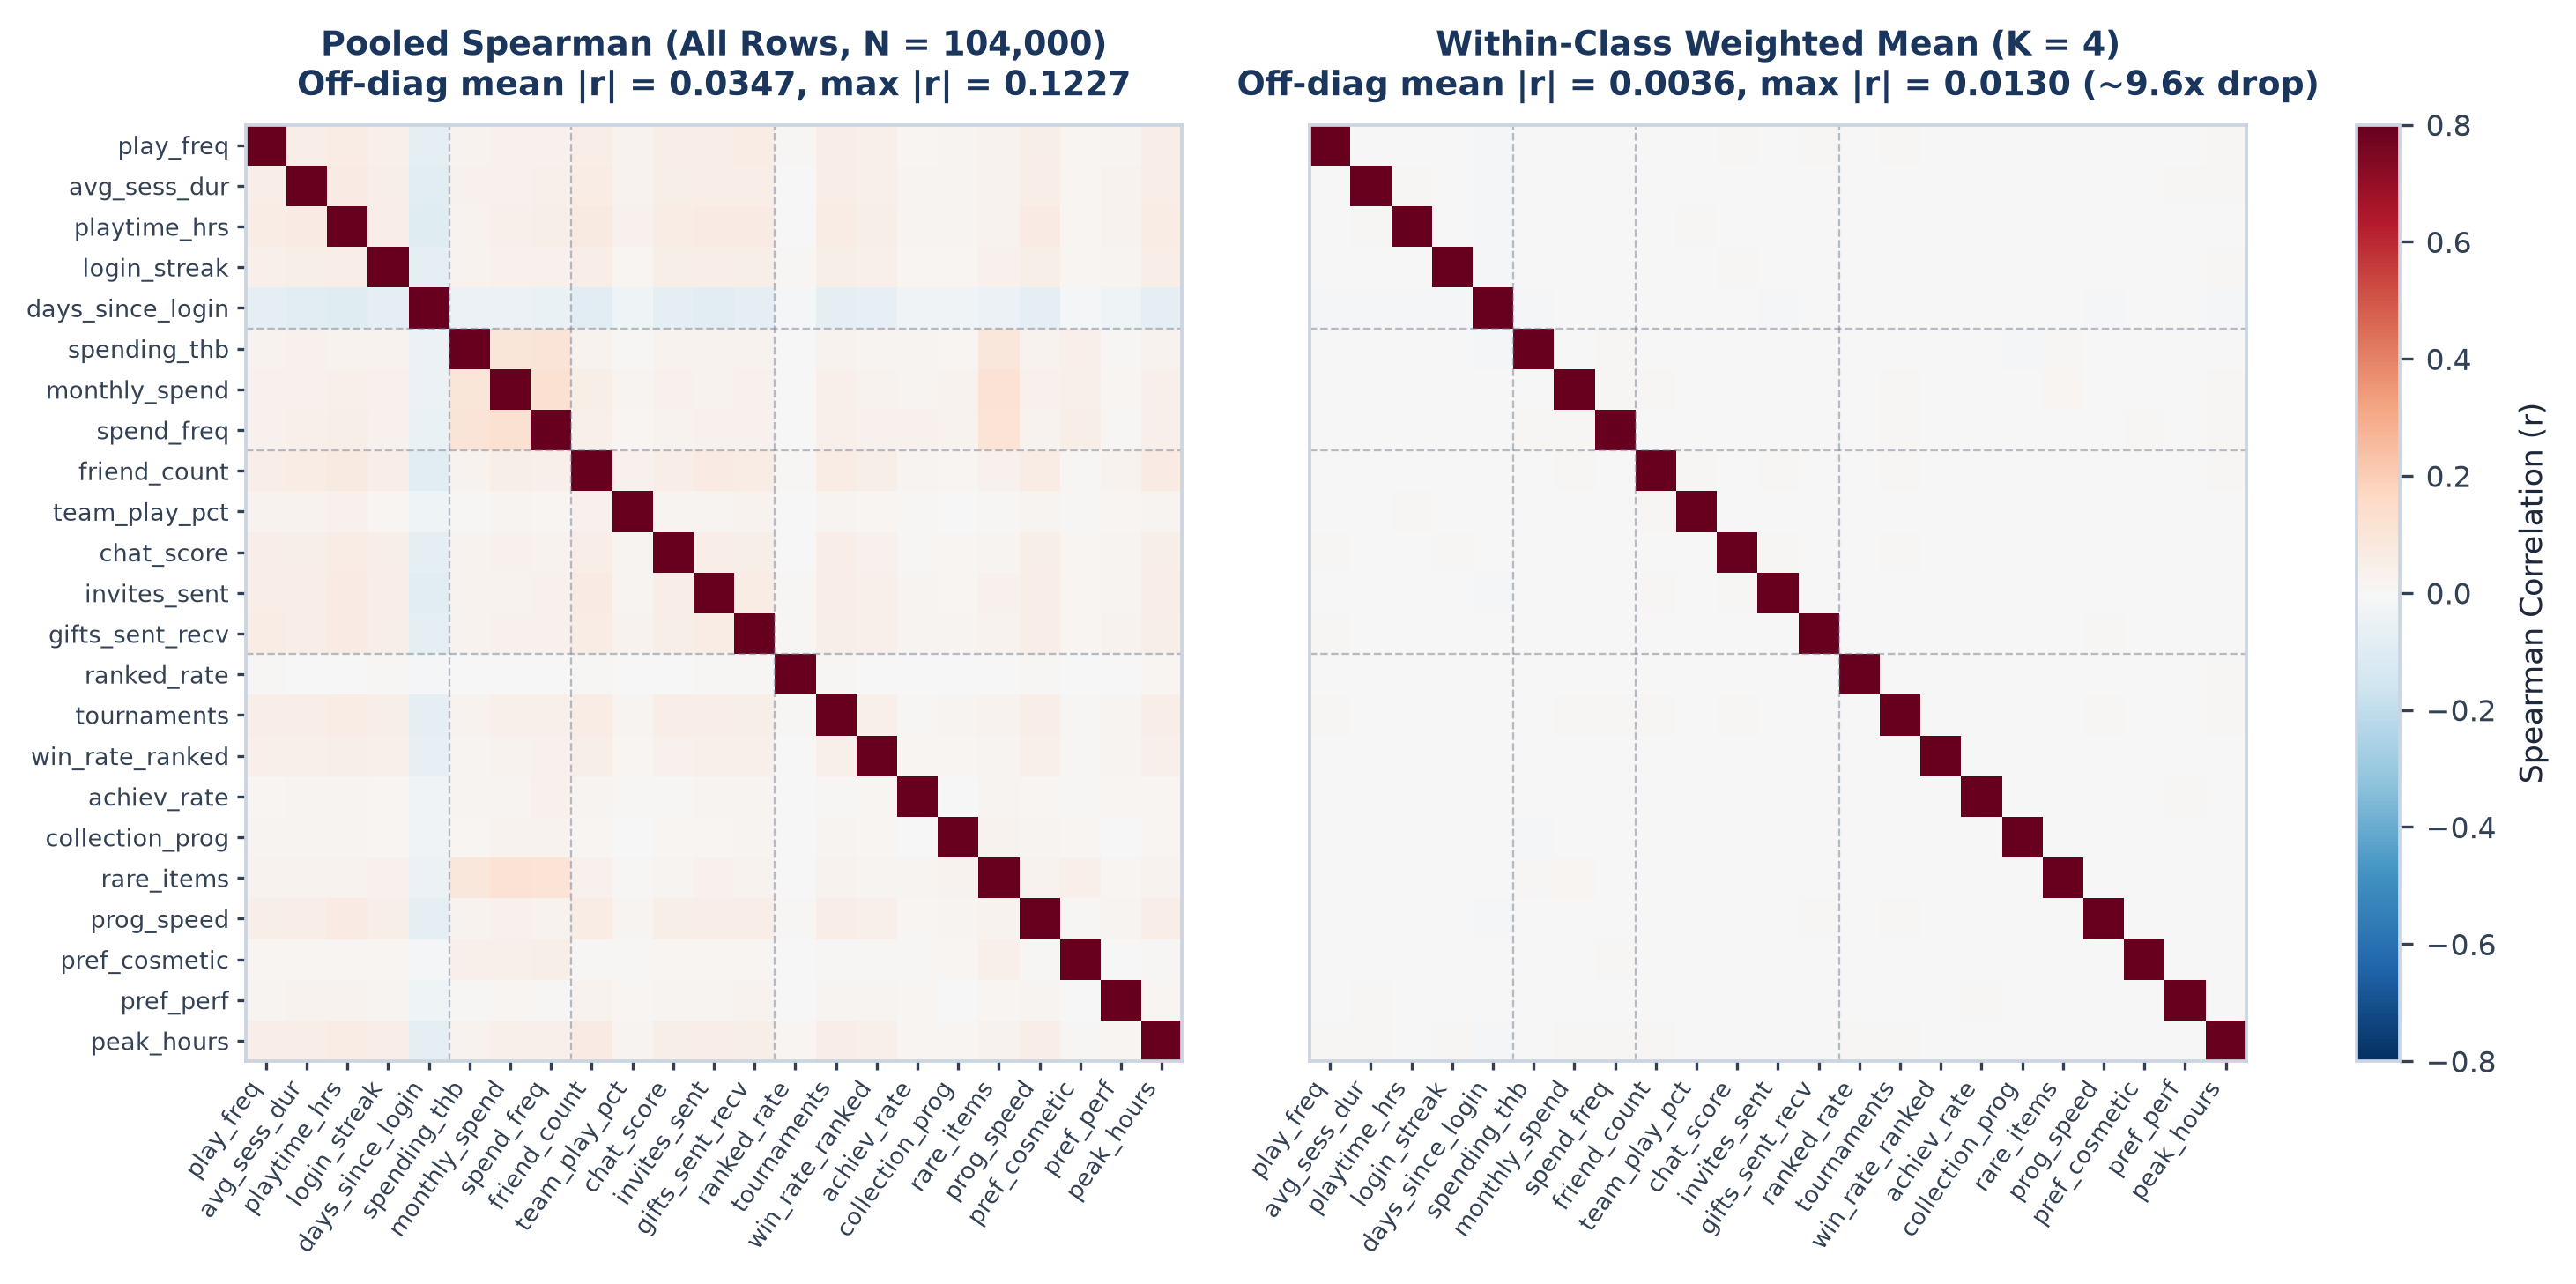
\includegraphics[width=\textwidth]{figures/t2/fig_t2_independence_heatmap.png}
  \caption{เปรียบเทียบเมทริกซ์สหสัมพันธ์ Spearman ของ 23 ฟีเจอร์ต่อเนื่องบนชุดฝึก v2 ($N = 104,000$): แผงซ้ายแสดงสหสัมพันธ์แบบรวมทุกแถว ($\mathrm{mean}\ |r| = 0.0347$, $\max |r| = 0.1227$) และแผงขวาแสดงค่าเฉลี่ยแบบถ่วงน้ำหนักภายในแต่ละคลาส ($\mathrm{mean}\ |r| = 0.0036$, $\max |r| = 0.0130$ หรือลดลงราว 9.6 เท่า) ยืนยันความเป็นอิสระเชิงมีเงื่อนไขของตัวแปร}
  \label{fig:t2_independence}
\end{figure}

\begin{figure}[htbp]
  \centering
  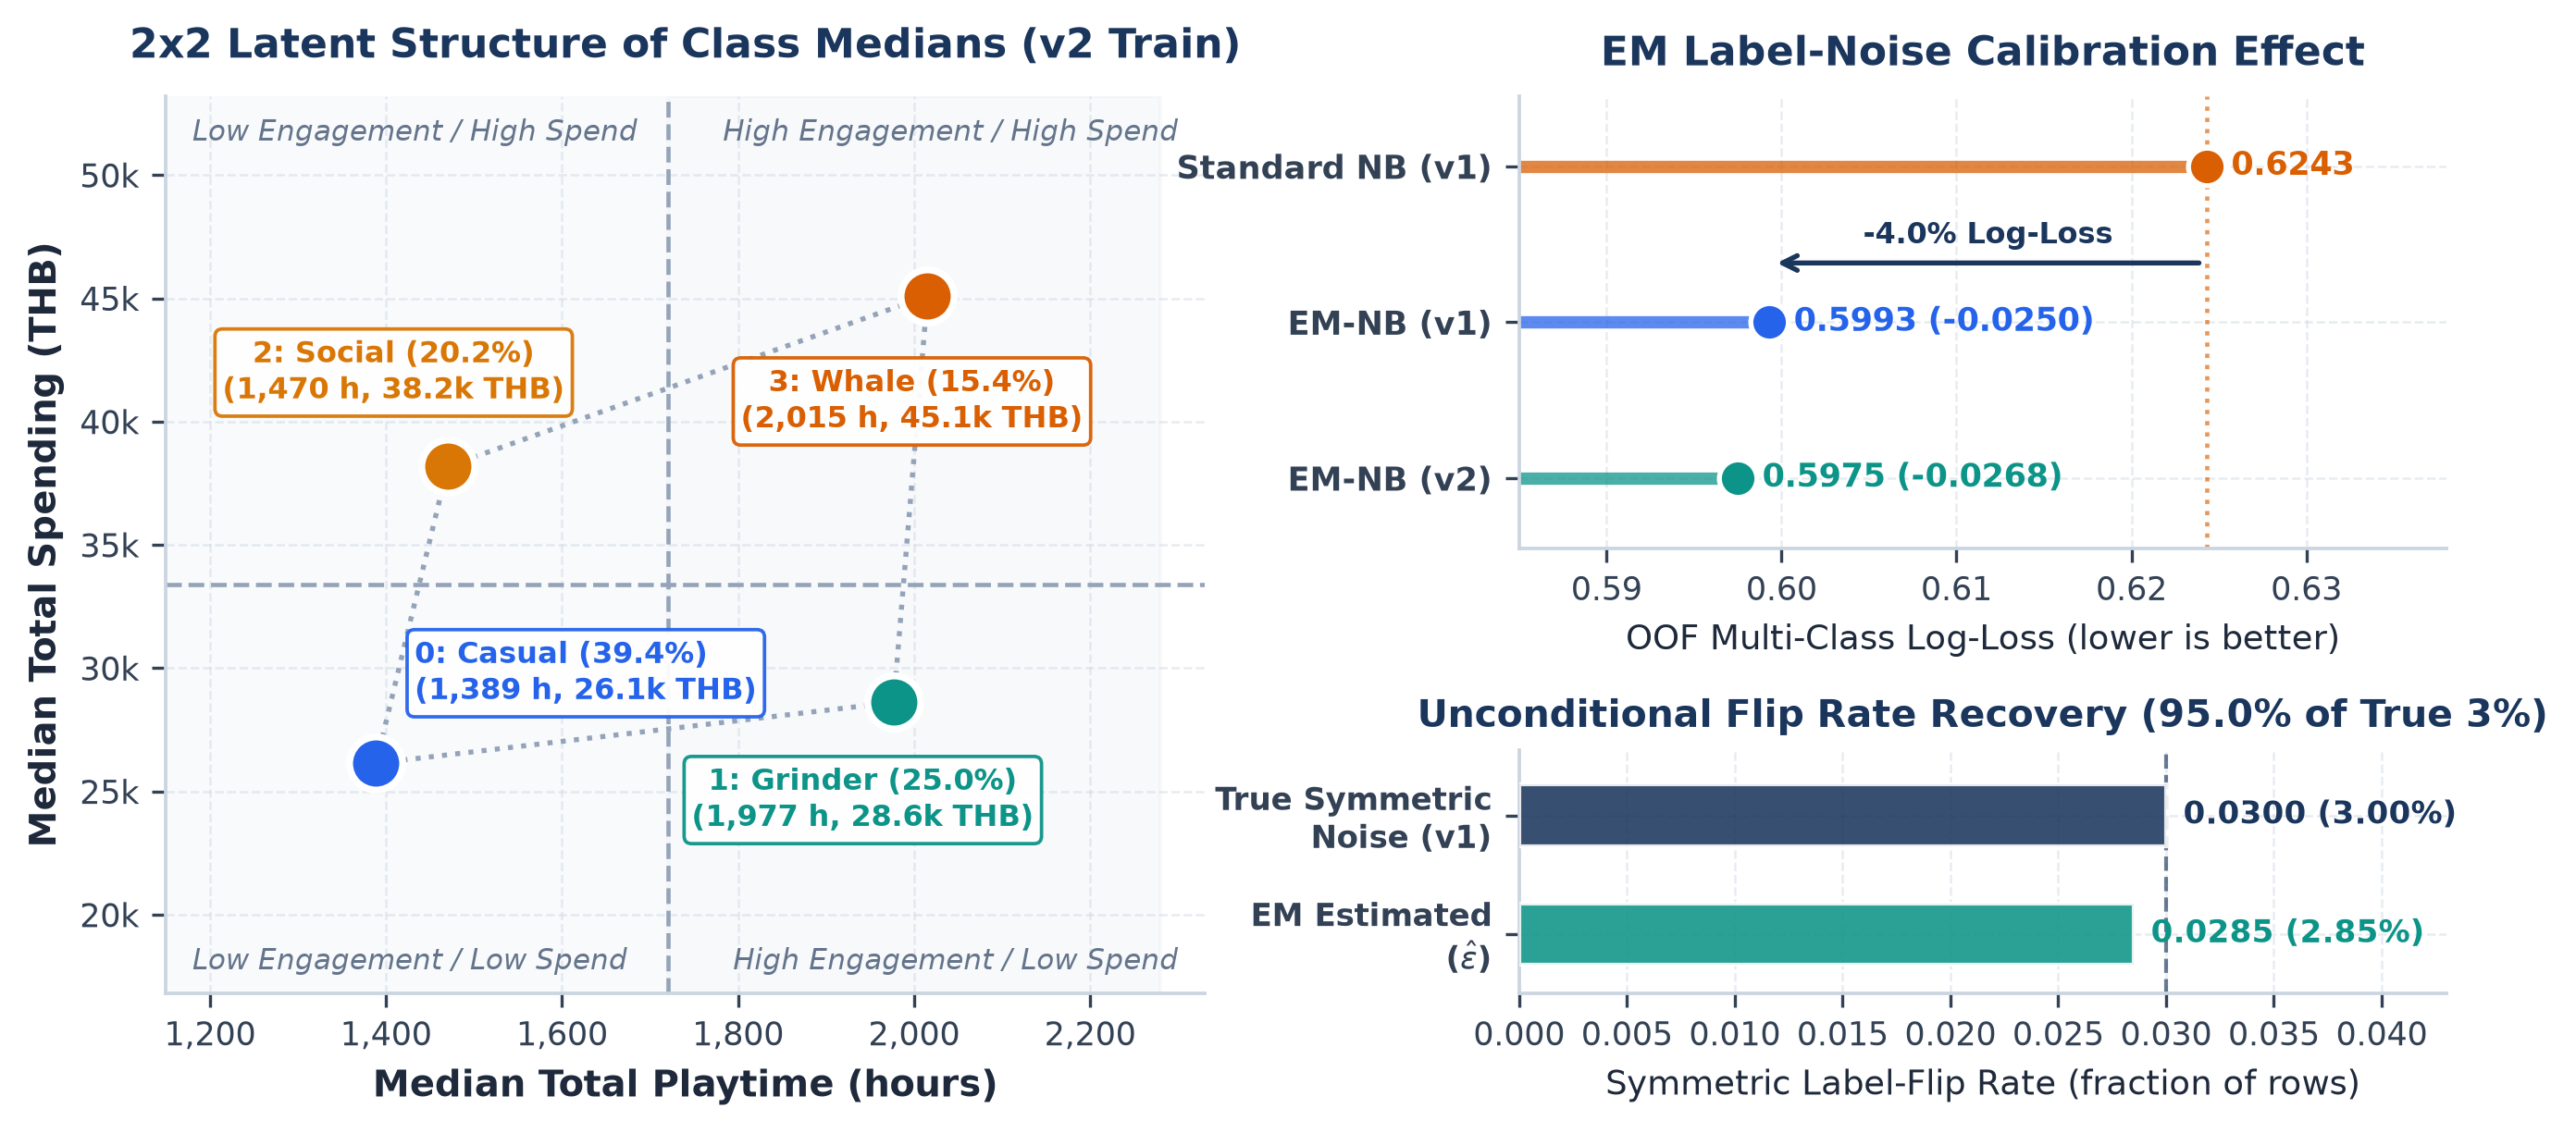
\includegraphics[width=\textwidth]{figures/t2/fig_t2_latent_2x2.png}
  \caption{แผงซ้าย: โครงสร้างแฝง $2 \times 2$ ของค่ามัธยฐาน \feat{total\_playtime\_hours} เทียบกับ \feat{total\_spending\_thb} บนชุดฝึก v2 แสดงความกำกวมระหว่างกลุ่ม Grinder กับ Whale หากพิจารณาเพียงชั่วโมงเล่น แผงขวาบน: ผลของการปรับเทียบความน่าจะเป็นด้วย EM Label-Noise Model ที่ลด Multi-Class Log-Loss ลงจาก 0.6243 เหลือ 0.5993 (v1) และ 0.5975 (v2) แผงขวาล่าง: การประมาณอัตราป้ายกำกับเพี้ยน $\hat{\varepsilon} = 0.0285$ เทียบกับค่าจริง 0.0300}
  \label{fig:t2_latent_2x2}
\end{figure}

% ==============================================================================
% PART 3: HISTOGRAM DENSITY & EM LABEL-NOISE MODEL
% ==============================================================================
\subsubsection{การเตรียมข้อมูล Histogram Density และโมเดล EM Label-Noise}
\label{subsubsec:t2_histogram_em}

ขั้นตอนการสร้างตาราง Log-Likelihood ของ Naive Bayes ได้รับการแก้ไขเชิงวิศวกรรมจากจุดบกพร่องสองประการในโค้ดตั้งต้น (\feat{t2/code/pf.py}) กล่าวคือ ประการแรก ฟังก์ชัน \feat{ll\_select} เดิมเปรียบเทียบค่า Histogram Log-\textit{Mass} ($\log P(\text{bin}_i \mid y_i)$) ข้ามจำนวนถังที่แตกต่างกัน ซึ่งความน่าจะเป็นรวมภายในหนึ่งถังย่อมสูงขึ้นเสมอเมื่อถังมีขนาดกว้างขึ้น ทำให้เกณฑ์นี้ลำเอียงเลือกถังหยาบ (coarse bins) โดยปริยาย ประการที่สอง การใช้ Optuna ปรับแต่งค่า $(\mathrm{nbins}, \sigma)$ ของทั้ง 23 ฟีเจอร์ต่อเนื่อง (46 ไฮเปอร์พารามิเตอร์ร่วมกับ $\alpha$) ด้วยเป้าหมาย $\mathrm{Macro}\ F_1$ แบบ 5-Fold CV บนแถวชุดเดิมซ้ำกันทุก trial ทำให้เกิดการโอเวอร์ฟิตเชิงโครงสร้าง แม้คะแนนแบบไม่ซ้อนจะดูสูงขึ้นเป็น 0.7557 แต่เมื่อตรวจสอบด้วย \textbf{Nested Optuna} (\feat{E13}: 150 TPE trials ภายใน 4-Fold inner CV ต่อ outer fold บน seed 42) คะแนนทดสอบจริงตกลงเหลือเพียง \textbf{0.7544} ซึ่งต่ำกว่าโมเดลพื้นฐานแบบไม่จูนที่ใช้ค่าคงที่ (32 bins, $\sigma = 0.7$, คะแนน 0.7550 หรือ 0.7548 บน fold เดียวกัน)

เพื่อขจัดทั้งอคติจากขนาดถังและความแปรปรวนจากการจูน $F_1$ เราจึงออกแบบระบบคัดเลือกความหนาแน่นแบบ \textbf{Inner-4-Fold Univariate Posterior Log-Loss} (\feat{t2/research/e14\_llselect.py} และ \feat{work/t2v2/make\_t2v2.py}) สำหรับฟีเจอร์ต่อเนื่อง $c \in \mathrm{CONT}$ ทั้ง 23 ตัว ขอบถังถูกสร้างจากควอนไทล์ของชุดฝึกเท่านั้น ($\mathrm{nanquantile}$) จากนั้นค้นหาคู่พารามิเตอร์ $(B, \sigma)$ จากกริด \feat{g2}: $B \in \{64, 128, 256\}$ และค่าเบี่ยงเบนมาตรฐานของการปรับเรียบแบบเกาส์เซียน $\sigma \in \{3.0, 4.0, 6.0, 8.0, 12.0\}$ (หน่วยความกว้างถัง) ร่วมกับการปรับเรียบ Laplace $\alpha = 1.0$ โดยประเมินค่าเฉลี่ย Univariate Posterior Log-Loss บน Inner 4-Fold Stratified CV:
\begin{equation}
\label{eq:t2_univariate_ll}
\mathcal{L}_{\mathrm{uni}}(c;\, B, \sigma) = -\frac{1}{|\mathcal{A}|}\sum_{(i \in \text{val})} \log \left[ \mathrm{softmax}\Big(\log \hat{\pi}_{\mathrm{train}} + \log \hat{p}_c(x_{ic} \mid \cdot\,; B, \sigma, \alpha=1)\Big) \right]_{y_i}
\end{equation}
เกณฑ์ในสมการ~(\ref{eq:t2_univariate_ll}) วัดความแม่นยำของความน่าจะเป็นหลังการสังเกต (posterior calibration) ต่อคลาสโดยตรง จึงเป็นอิสระจากการหดหรือขยายความกว้างของถัง (invariant to bin width) และมีค่าความแปรปรวนต่ำมากโดยไม่ต้องปรับแต่งบน $\mathrm{Macro}\ F_1$ ผลลัพธ์ที่ได้คือตัวแบบเลือกใช้ความละเอียดสูงขึ้นและการปรับเรียบที่นุ่มนวลขึ้น (64--256 bins, $\sigma \in [3, 12]$) ทั้งนี้กริดเริ่มต้น \feat{g1} ($8\text{--}128$ bins, $\sigma \in [0, 4]$) พบว่าค่าที่เลือกมักชนขอบบนที่ 128 bins และ $\sigma=4$ ขณะที่กริดที่ขยายไกลกว่านั้นอย่าง \feat{g3} ($128\text{--}512$ bins, $\sigma \in [6, 24]$) เกิดการเบลอมากเกินไป (over-smoothing) จนคะแนนลดลงเหลือ 0.7557 บน seed 42 ดังนั้นกริด \feat{g2} จึงเป็นจุดสมดุลที่เหมาะสมที่สุด

ถัดจากขั้นตอนการสร้างถังข้อมูล เราจำลองความจริงที่ว่าป้ายกำกับที่สังเกต $\tilde{y}_i$ มีสัญญาณรบกวนสมมาตรด้วย \textbf{Expectation-Maximization Naive Bayes (EM-NB)} (\feat{e06\_emnb.py}) โดยกำหนดให้แต่ละผู้เล่นมีคลาสแฝงที่แท้จริง $z_i \in \{0, 1, 2, 3\}$ ด้วยสัดส่วนเริ่มต้น $\pi_z$ และมีเมทริกซ์เปลี่ยนผ่านสัญญาณรบกวน $M_\varepsilon \in \mathbb{R}^{4 \times 4}$ ที่กำหนดความน่าจะเป็นแบบสมมาตรว่า $P(\tilde{y}=k \mid z=z) = 1 - \varepsilon$ และ $P(\tilde{y}=k \mid z \neq k) = \varepsilon / 3$ อัลกอริทึม EM ทำงานซ้ำจำนวน 15 รอบ (เริ่มจาก $\varepsilon^{(0)} = 0.03$) ดังนี้:
\begin{itemize}
  \item \textbf{E-step (คำนวณความรับผิดชอบของคลาสแฝง):} สำหรับแต่ละแถวฝึก $i$ คำนวณความน่าจะเป็นภายหลังของคลาสแฝง $z$ จากผลคูณความน่าจะเป็นของฟีเจอร์ที่มีค่าและโอกาสของป้ายกำกับที่สังเกต:
  \begin{equation}
  \label{eq:t2_estep}
  r_{iz}^{(t)} = \mathrm{softmax}_z\!\left(\log \pi_z^{(t)} + \sum_{j:\, x_{ij} \neq \mathrm{NaN}} \log p_j^{(t)}(x_{ij} \mid z) + \log P(\tilde{y}_i \mid z;\, \varepsilon^{(t)})\right)
  \end{equation}
  \item \textbf{M-step (ปรับปรุงพารามิเตอร์แบบถ่วงน้ำหนักอ่อน):} อัปเดตความถี่ในแต่ละถังด้วยน้ำหนัก $r_{iz}^{(t)}$ ผ่านตัวกรองเกาส์เซียนและ $\alpha=1$ (โดยไม่รวมตัวอย่างที่ฟีเจอร์ต่อเนื่องเป็น \feat{NaN}) เพื่อสร้างตาราง $\log p_j^{(t+1)}(b \mid z)$ พร้อมทั้งปรับค่าสัดส่วนคลาสแฝง $\pi_z^{(t+1)} = \frac{1}{N}\sum_{i=1}^N r_{iz}^{(t)}$ และประมาณอัตราการสลับป้ายกำกับใหม่ $\hat{\varepsilon}^{(t+1)} = 1 - \frac{1}{N}\sum_{i=1}^N r_{i,\tilde{y}_i}^{(t)}$
  \item \textbf{Prediction (พยากรณ์ความน่าจะเป็นของป้ายกำกับที่สังเกต):} เมื่อทำนายข้อมูลนอกกลุ่มฝึกหรือชุดทดสอบ ความน่าจะเป็นของป้ายกำกับ $\tilde{y}$ จะถูกฉายผ่านเมทริกซ์สัญญาณรบกวน:
  \begin{equation}
  \label{eq:t2_em_pred}
  P(\tilde{y} \mid x) = \mathrm{softmax}\!\left(\log \hat{\pi} + \sum_{j:\, x_j \neq \mathrm{NaN}} \log \hat{p}_j(x_j \mid \cdot)\right) \cdot M_{\hat{\varepsilon}}
  \end{equation}
\end{itemize}
การจำลองสัญญาณรบกวนแบบ EM นี้ช่วยแยกตัวอย่าง 3\% ที่ป้ายกำกับเพี้ยนออกจากการบิดเบือนตารางความหนาแน่นและทำให้ค่าความน่าจะเป็นที่พยากรณ์ถูกปรับเทียบอย่างแม่นยำ ส่งผลให้ OOF Multi-Class Log-Loss ลดลงจาก \textbf{0.6243} ใน Standard NB (v1) เหลือ \textbf{0.5993} ใน EM-NB (v1) และลดลงถึง \textbf{0.5975} บนชุดข้อมูล v2 (ลดลงกว่า 4\% ดังภาพประกอบในรูปที่~\ref{fig:t2_latent_2x2})

% ==============================================================================
% PART 4: BLEND & AFFINE F1 DECISION RULE
% ==============================================================================
\subsubsection{การออกแบบโมเดล Blend และกฎตัดสินใจ Affine สำหรับ Macro $F_1$}
\label{subsubsec:t2_blend_affine}

การเปรียบเทียบตระกูลโมเดลที่หลากหลายยืนยันว่าโมเดลเชิงสร้าง EM-NB เอาชนะโมเดลเชิงจำแนกทุกกลุ่มอย่างสม่ำเสมอ โมเดล LightGBM แบบพื้นฐานได้ Train in-sample $\mathrm{Macro}\ F_1 = 0.7925$ แต่กลับได้ผลบน OOF เพียง 0.7509 (แบบ raw) และ 0.7524 (หลังจูนด้วย Nested Optuna ใน \feat{E17b}) คิดเป็น Overfit Gap สูงถึง $+0.0416$ เทียบกับ EM-NB ที่มีช่องว่างเพียง $+0.0016$ (0.7578 บนชุดฝึก vs 0.7562 บน OOF ใน v1 ดังแสดงในรูปที่~\ref{fig:t2_progression_overfit} แผงซ้าย) สาเหตุเนื่องจากต้นไม้ตัดสินใจต้องสร้างขอบเขตแบบขั้นบันไดตามแนวแกนจำนวนมากเพื่อเลียนแบบเส้นโค้งความน่าจะเป็นที่เรียบและเป็นอิสระใน 23 มิติ ส่วน ExtraTrees (0.7057), QDA (0.6757), LDA (0.7336), กลุ่ม SVM (0.7304--0.7406) และโมเดลผู้เชี่ยวชาญเฉพาะคลาสแบบ One-vs-Rest (\feat{E15}: 0.7537--0.7551) ต่างมีอคติเชิงโครงสร้างหรือความแปรปรวนที่สูงกว่า

อย่างไรก็ตาม การผสานโมเดลต่างตระกูลที่อาศัยสถาปัตยกรรมแบบบวกหรือเรียบต่อเนื่องช่วยลดความแปรปรวนบริเวณรอยต่อของคลาสได้เล็กน้อย เราจึงสร้าง Ensemble แบบ Controlled Diversity Blend บนชุดข้อมูล v2 โดยถ่วงน้ำหนัก:
\begin{equation}
\label{eq:t2_blend}
P_{\mathrm{blend}}(x) = 0.87\,P_{\mathrm{EM\text{-}NB}}(x) + 0.08\,P_{\mathrm{Spline\text{-}LR}}(x) + 0.05\,P_{\mathrm{MLP}}(x)
\end{equation}
โดยที่องค์ประกอบเชิงจำแนกทั้งสองตัวฝึกจาก 28 ฟีเจอร์ที่คัดกรองแล้ว (ปราศจาก \feat{player\_id}) ได้แก่ (1) \textbf{Spline Logistic Regression} (\feat{logreg\_spline\_A}, OOF $\mathrm{Macro}\ F_1 = 0.75468$, Log-Loss $0.62143$) ซึ่งแปลงฟีเจอร์ต่อเนื่องผ่าน \feat{QuantileTransformer(normal)} และ \feat{StandardScaler} ตามด้วย \feat{SplineTransformer(n\_knots=6, degree=3)} ร่วมกับ one-hot ของ \feat{engagement\_level} และ \feat{loyalty\_tier} แล้วฝึกด้วย \feat{LogisticRegression(C=0.05)} และ (2) \textbf{PyTorch Tabular MLP} (\feat{mlp\_torch\_A}, OOF $\mathrm{Macro}\ F_1 = 0.75227$, Log-Loss $0.61075$) โครงข่าย 3 ชั้น (\texttt{128 $\to$ 64 $\to$ 4}) ที่ใช้ฟังก์ชันกระตุ้น \feat{SiLU}, \feat{Dropout(0.2)}, \feat{AdamW(lr=2e-3, wd=1e-3)} และ \feat{OneCycleLR} เป็นเวลา 12 epochs

เหตุผลสำคัญที่คงค่าน้ำหนัก \texttt{0.87 / 0.08 / 0.05} (สอดคล้องกับผล Nested Log-Loss Weighting ใน \feat{E16} ของ v1 ที่เลือก EM-NB $\approx 0.878$ ร่วมกับ GAM $\approx 0.110$) มาจากการทดสอบ \feat{work/t2v2/tune\_blend.py} แบบ Nested $3 \times 5$-Fold CV บน v2: แม้การค้นหาบน OOF ทั้งชุดจะให้น้ำหนัก $(0.60, 0.35, 0.05)$ ที่คะแนน $0.7588$ แต่เมื่อประเมินแบบ Nested เต็มรูปแบบ น้ำหนักที่จูนใหม่ได้คะแนนเฉลี่ย $0.75833$ เทียบกับ $0.75826$ ของน้ำหนัก \texttt{0.87 / 0.08 / 0.05} คิดเป็นผลต่างเพียง $+0.00006 \pm 0.00018$ (ชนะ 8 จาก 15 folds) ซึ่งอยู่ในระดับสัญญาณรบกวนสุ่ม การยึดน้ำหนักเดิมจึงช่วยป้องกันการโอเวอร์ฟิตน้ำหนัก Blend ต่อ OOF ได้อย่างมีประสิทธิภาพ

เมื่อได้ความน่าจะเป็นรวม $p_k(x) = [P_{\mathrm{blend}}(x)]_k$ ที่ปรับเทียบดีแล้ว ขั้นสุดท้ายคือการแปลงความน่าจะเป็นให้เป็นการตัดสินใจเชิงคลาสที่เหมาะสมที่สุดสำหรับ $\mathrm{Macro}\ F_1$ แทนการใช้ $\arg\max$ แบบเดิม

\begin{decisionbox}[กฎตัดสินใจ Fixed-Point Affine $F_1$ สำหรับ Macro $F_1$]
จากการหาอนุพันธ์เชิงฟังก์ชันของ $\mathrm{Macro}\ F_1$ ในสมการ~(\ref{eq:t2_macro_f1}) รอบจุดสมดุล $(q_k, F_k)$ เมื่อกำหนดให้ตัวอย่าง $x$ ได้รับการทำนายเป็นคลาส $k$ ตัวเศษ $2\,\mathbb{P}(y=k, \hat{y}=k)$ จะเพิ่มขึ้นเท่ากับ $2\,p_k(x)$ ขณะที่สัดส่วนการทำนาย $q_k$ ในตัวหารเพิ่มขึ้น $1$ ก่อให้เกิดผลกระทบเชิงลบอัตรา $\frac{\partial F_{1,k}}{\partial q_k} = \frac{-F_k}{\pi_k + q_k}$ ดังนั้น การเลือกคลาสที่ให้ค่าเพิ่มเชิงเส้นสูงสุดของ $\sum_k F_{1,k}$ จึงลดรูปเป็นกฎตัดสินใจแบบ \textbf{Affine} ($\hat{y}(x) = \arg\max_k (a_k\,p_k(x) + b_k)$) โดยที่:
\begin{equation}
\label{eq:t2_affine_rule}
a_k = \frac{2}{\pi_k + q_k}, \qquad b_k = \frac{-F_k}{\pi_k + q_k}
\end{equation}
ในสคริปต์ \feat{work/t2v2/make\_t2v2.py} แก้สมการจุดตรึง (fixed-point iteration) จำนวน 8 รอบโดยเริ่มต้นที่ $q^{(0)} = \pi$ และ $F^{(0)} = 0.75$ ทุกคลาส แล้วปรับค่า $q_k$ และ $F_k$ จากผลทำนาย $\arg\max_k (a_k p_{ik} + b_k)$ บน OOF จนลู่เข้าได้สัมประสิทธิ์ $a = [2.4967,\; 3.9800,\; 5.0020,\; 6.7430]$ และ $b = [-1.0241,\; -1.4889,\; -1.7933,\; -2.5199]$ (กับ $q = [0.4072,\; 0.2522,\; 0.1976,\; 0.1429]$) กฎนี้ช่วยเพิ่มน้ำหนักให้คลาสที่มีตัวหาร $\pi_k+q_k$ เล็กอย่าง Social และ Whale บริเวณขอบเขตที่กำกวม โดยแลก $F_{1,0}$ ของ Casual ลงเล็กน้อย (0.82387 $\to$ 0.82037) เพื่อยกระดับ Grinder (0.74649 $\to$ 0.74817), Social (0.71542 $\to$ 0.71704) และ Whale (0.74613 $\to$ 0.74747) ทำให้ $\mathrm{Macro}\ F_1$ เพิ่มจาก 0.75798 เป็น \textbf{0.75826} (+0.00028) โดยปรับเปลี่ยนเฉพาะแถวขอบเขต 2,056 / 104,000 แถว (1.98\%)
\end{decisionbox}

% ==============================================================================
% PART 5: VALIDATION STRATEGY, EXPERIMENT PROGRESSION & FINAL RESULTS
% ==============================================================================
\subsubsection{กลยุทธ์การวัดผล ลำดับการทดลอง และผลลัพธ์สุดท้าย (v1 และ v2 Re-Release)}
\label{subsubsec:t2_validation_results}

กลยุทธ์การวัดผลใช้ \textbf{5-Fold StratifiedKFold} ซ้ำ 3 seeds (42, 7, 123) เพื่อวัดเสถียรภาพของโครงสร้างโมเดล โดยทุกขั้นตอนที่เกี่ยวข้องกับป้ายกำกับ (การคัดเลือกกริด $(\mathrm{nbins}, \sigma)$, การฝึก EM, โมเดล meta-learner และกฎตัดสินใจในฝั่งวิจัย) ต้องทำแบบ Nested ภายใน outer training folds เสมอ เพื่อขจัดอคติเชิงบวกเกินจริง ทั้งนี้ค่าความผันผวนจากการสุ่มตัวอย่างของ $\mathrm{Macro}\ F_1$ บนชุดข้อมูลขนาดแสนแถวอยู่ที่ประมาณ $\pm 0.002$ (SD ระหว่าง fold ในหนึ่ง seed $\approx 0.0021\text{--}0.0024$)

ตารางที่~\ref{tab:t2_v1_benchmark} สรุปผลการทดลองเปรียบเทียบเชิงลึกบนชุดข้อมูล v1 (\feat{E00--E17} และ \feat{blind\_sonnet}) ซึ่งพิสูจน์ข้อได้เปรียบของสถาปัตยกรรม EM-NB ที่คัดเลือกความหนาแน่นด้วย Log-Loss เหนือทุกตระกูลโมเดล จากนั้นเรานำสูตรสำเร็จเดียวกันมาสร้างและตรวจสอบบนชุดข้อมูล v2 ที่ปราศจากการรั่วไหล (\feat{work/t2v2/make\_t2v2.py}) ดังแสดงลำดับความก้าวหน้าในตารางที่~\ref{tab:t2_v2_progression} และรูปที่~\ref{fig:t2_progression_overfit}

\begin{table}[htbp]
  \centering
  \caption{ตารางเปรียบเทียบผลการทดลองเชิงโครงสร้างบนชุดข้อมูล v1 (Feature-Only ยกเว้นแถวอ้างอิง Leak, 5-Fold Stratified CV)}
  \label{tab:t2_v1_benchmark}
  {\scriptsize
  \begin{tabularx}{\textwidth}{@{}l p{4.2cm} r r X@{}}
    \toprule
    \textbf{รหัส} & \textbf{โมเดล / การทดลอง} & \textbf{Macro $F_1$} & \textbf{Log-Loss} & \textbf{ข้อสรุปเชิงวิศวกรรม} \\
    \midrule
    \feat{E00} & NB Uniform (32 bins, $\sigma=0.7$) & 0.7550 $\pm$ 0.0004 & --- & Baseline อิสระ (Train 0.7582) \\
    \feat{E00} & NB Optuna (ไม่ซ้อน Folds) & 0.7557 $\pm$ 0.0004 & 0.6243 & โอเวอร์ฟิต 46 พารามิเตอร์ (ดู \feat{E13}) \\
    \feat{E13} & NB Nested Optuna (seed 42) & 0.7544 & --- & ต่ำกว่า Uniform (0.7548 on s42) \\
    \feat{E14 g1} & NB LL-select (bins 8--128, $\sigma$ 0--4) & 0.7554 $\pm$ 0.0001 & 0.6229 & ชนขอบกริดที่ 128 bins และ $\sigma=4$ \\
    \feat{E14 g2} & NB LL-select (bins 64--256, $\sigma$ 3--12) & 0.7558 $\pm$ 0.0002 & 0.6229 & +0.0014 เหนือ Nested Optuna \\
    \textbf{\feat{E14 g2+EM}} & \textbf{EM-NB + LL-select (Final v1)} & \textbf{0.7562 $\pm$ 0.0002} & \textbf{0.5993} & \textbf{Train 0.7578, Gap +0.0016} \\
    \feat{E17a} & Nested Optuna on EM-NB (LL) & 0.7562 & 0.5992 & เสมอตัว จึงคงค่าเริ่มต้นเดิม \\
    \feat{E16} & Nested Blend (\feat{lin\_ll}, 6 โมเดล) & 0.7563 $\pm$ 0.0001 & 0.5991 & เลือก EM-NB 0.878 + GAM 0.110 \\
    \midrule
    \feat{E02} & Multinomial Spline-GAM ($k=8$) & 0.7529 $\pm$ 0.0005 & 0.6198 & เส้นโค้งจำแนกแม่นน้อยกว่า NB \\
    \feat{E12} & Spline-GAM + Noise Corr. ($\hat{\varepsilon}=0.027$) & 0.7525 & 0.6029 & แก้ LL ได้ แต่ความแม่นยำยังต่ำกว่า \\
    \feat{E04} & WANBIA (\feat{w / wk / LR}, s42) & 0.7539--0.7542 & 0.6195--0.6207 & การถ่วงน้ำหนักฟีเจอร์ไม่ช่วยเพิ่ม \\
    \feat{E05/E17b} & LightGBM (\feat{raw} / \feat{tuned}, s42) & 0.7509 / 0.7524 & 0.6173 / 0.6170 & Train 0.7925 (Gap +0.0416) \\
    \feat{E15} & Class Specialists (OvR LightGBM) & 0.7537--0.7551 & --- & AUC เท่า NB (0.931/0.923/0.924/0.940) \\
    \feat{blind} & Spline LR / PyTorch MLP & 0.7521 / 0.7511 & --- & องค์ประกอบ diversity ที่ดีที่สุด \\
    \feat{blind} & SVM Nyström / Linear / RBF & 0.7406 / 0.7304 / 0.7395 & --- & ด้อยกว่าโครงสร้างเชิงบวกอิสระ \\
    \feat{blind} & LDA / ExtraTrees / QDA & 0.7336 / 0.7057 / 0.6757 & --- & ต้นไม้สุ่ม/ความแปรปรวนร่วมเต็มรูปไม่เหมาะ \\
    \midrule
    \feat{E10} & \feat{player\_id} Block Rule (v1 Leak) & 0.9677 $\pm$ 0.0000 & 0.168 & เพดานจาก ID leak (ถูกกำจัดใน v2) \\
    \bottomrule
  \end{tabularx}}
\end{table}

\begin{table}[htbp]
  \centering
  \caption{ลำดับความก้าวหน้าของโมเดล Feature-Only บนชุดข้อมูล v2 (12 พ.ย., ปราศจาก \feat{player\_id}) และการกระจายตัวของคำทำนายสุดท้ายบน Test ($N = 25,889$)}
  \label{tab:t2_v2_progression}
  {\footnotesize
  \begin{tabularx}{\textwidth}{@{}X r r p{4.7cm}@{}}
    \toprule
    \textbf{ขั้นตอนโมเดล (v2 Clean OOF)} & \textbf{Macro $F_1$} & \textbf{$\Delta$ ขั้นก่อนหน้า} & \textbf{รายละเอียด / Log-Loss} \\
    \midrule
    QDA (\feat{qda\_A}) & 0.6754 & --- & SD 0.0018 (ความแปรปรวนพารามิเตอร์สูง) \\
    LDA (\feat{lda\_A}) & 0.7337 & --- & SD 0.0043 (ขอบเขตเชิงเส้นไม่เพียงพอ) \\
    \midrule
    PyTorch MLP (\feat{mlp\_torch\_A}) & 0.75227 & --- & 3-layer SiLU, Log-Loss 0.61075 \\
    Spline Logistic Regression (\feat{logreg\_spline\_A}) & 0.75468 & +0.00241 & 6-knot quantile splines, Log-Loss 0.62143 \\
    EM-NB (LL-selected, seed 42) & 0.75766 & +0.00298 & Log-Loss \textbf{0.5975} (3 seeds: 0.7577/0.7582/0.7578) \\
    Blend (0.87 NB / 0.08 LR / 0.05 MLP) Argmax & 0.75798 & +0.00032 & Log-Loss 0.59766 \\
    \textbf{Blend + Fixed-Point Affine Rule (Final)} & \textbf{0.75826} & \textbf{+0.00028} & \textbf{ปรับ 2,056 OOF rows (1.98\%)} \\
    \midrule
    \multicolumn{4}{@{}p{\textwidth}@{}}{\textbf{การกระจายคลาสสุดท้ายบนชุดทดสอบ (\feat{t2v2\_blend\_affine.csv} / \feat{sub\_v85a}, $N=25,889$):}} \\
    \multicolumn{4}{@{}p{\textwidth}@{}}{0: Casual = 10,576 (40.85\%) \quad|\quad 1: Grinder = 6,578 (25.41\%) \quad|\quad 2: Social = 5,020 (19.39\%) \quad|\quad 3: Whale = 3,715 (14.35\%)} \\
    \bottomrule
  \end{tabularx}}
\end{table}

\begin{figure}[htbp]
  \centering
  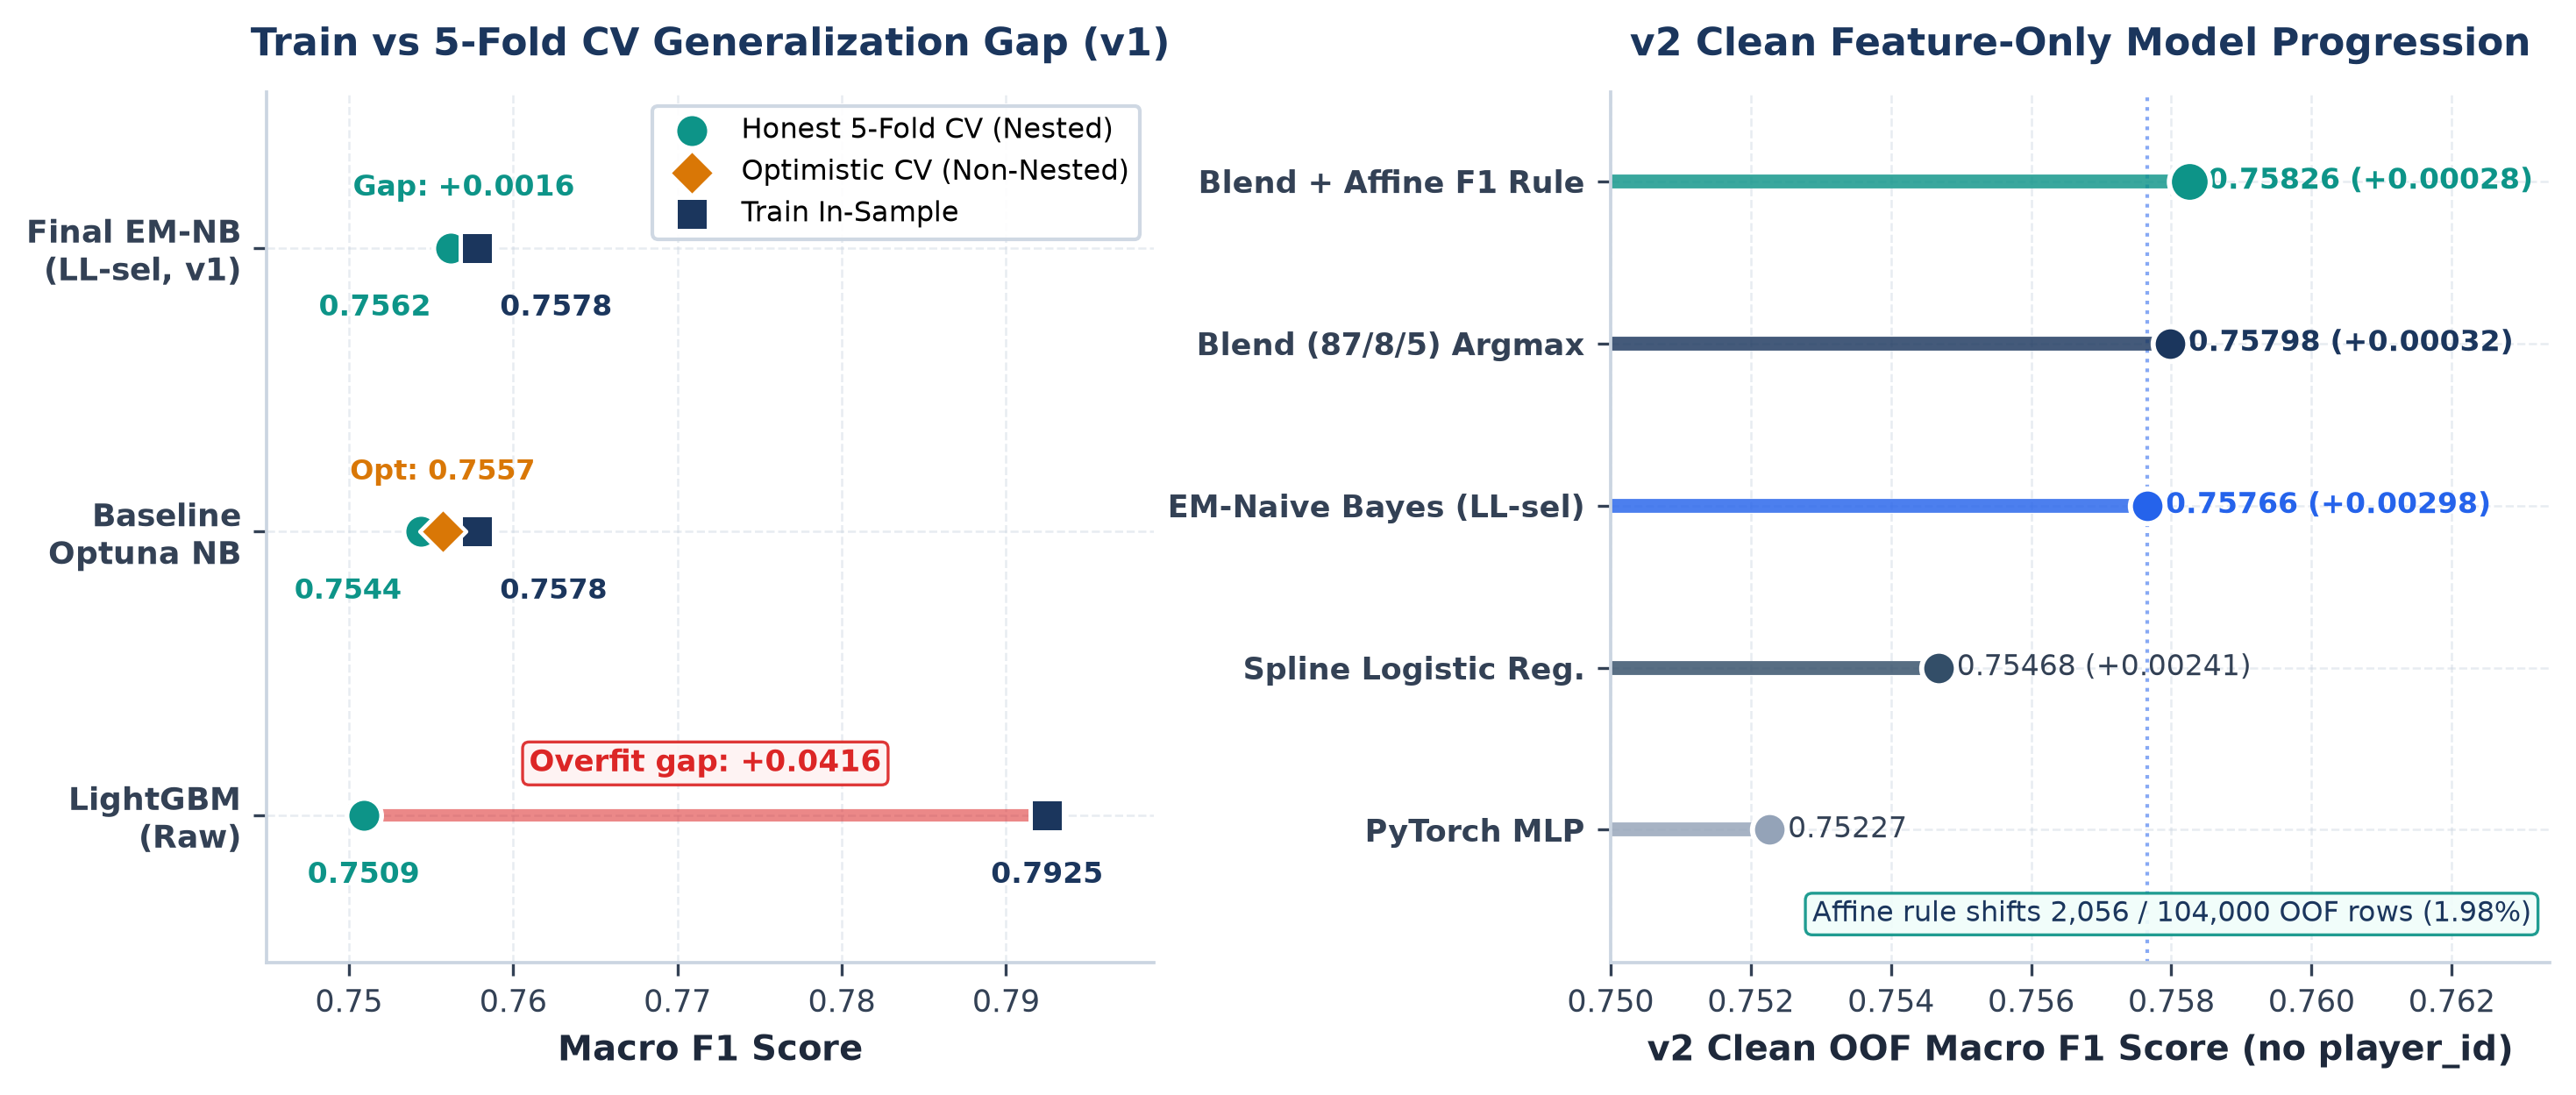
\includegraphics[width=\textwidth]{figures/t2/fig_t2_progression_and_overfit.png}
  \caption{แผงซ้าย: การวินิจฉัย Overfitting บนชุดข้อมูล v1 เปรียบเทียบคะแนน Train กับ Honest Nested CV พบว่า LightGBM มีช่องว่างถึง +0.0416 และ Baseline Optuna มีความลำเอียง +0.0013 ขณะที่ EM-NB (LL-sel) มีช่องว่างเพียง +0.0016 แผงขวา: พัฒนาการของคะแนน OOF $\mathrm{Macro}\ F_1$ บนชุดข้อมูล v2 ที่ปราศจาก \feat{player\_id} ตั้งแต่ MLP (0.75227) จนถึง Blend + Affine $F_1$ Rule (0.75826)}
  \label{fig:t2_progression_overfit}
\end{figure}

สำหรับผลยืนยันบน Public Leaderboard ก่อนการออกชุดข้อมูลใหม่ พบว่าเมื่อเปลี่ยนเฉพาะส่วน Task 2 จากโมเดล EM-NB เดี่ยว (\feat{sub\_v16b}: 0.71965) เป็นสถาปัตยกรรม 3-Model Blend + Fixed-Point Affine Rule (\feat{sub\_v18a}: 0.71999) คะแนนรวมเพิ่มขึ้น \textbf{+0.00034} (คิดเป็นผลต่างราว \textbf{+0.0017} เฉพาะส่วน Task 2) และในชุดทดสอบ v2 กฎ Affine ดังกล่าวปรับเปลี่ยนคำทำนายต่างจาก \feat{t2v2\_nb.csv} จำนวน 502 แถว โดยมีสัดส่วนคลาสทดสอบ (40.85\%, 25.41\%, 19.39\%, 14.35\%) สอดคล้องอย่างแนบแน่นกับจุดสมดุล $q$ จาก OOF และถูกบรรจุเข้าสู่ไฟล์ส่งงานสุดท้าย (\feat{submissions/FINAL/sub\_v85a\_soup\_trainprior.csv}) อย่างสมบูรณ์

% ==============================================================================
% PART 6: PLAYER_ID LEAK TRANSPARENCY, FAILED EXPERIMENTS & DATA CEILING
% ==============================================================================
\subsubsection{ความโปร่งใสเรื่อง \feat{player\_id} Leak การทดลองที่ไม่ได้ผล และเพดานของข้อมูล}
\label{subsubsec:t2_leak_failures_ceiling}

\begin{warningbox}[ความโปร่งใสด้านข้อมูล: การรั่วไหลของ \feat{player\_id} และการแก้ไขในฉบับ Re-Release (12 พ.ย.)]
ในชุดข้อมูล v1 ก่อนวันที่ 12 พฤศจิกายน รหัสผู้เล่น \feat{player\_id} (\feat{P000000}--\feat{P129999}) ถูกกำหนดเรียงตามลำดับบล็อกของคลาสที่แท้จริงในอัตราส่วน 40 / 25 / 20 / 15\% โดยมีจุดตัดที่แน่นอนคือ 0--51,999 $\to$ 0, 52,000--84,499 $\to$ 1, 84,500--110,499 $\to$ 2 และ 110,500--129,999 $\to$ 3 การใช้กฎบล็อก ID (\feat{E10}) ทำคะแนน OOF $\mathrm{Macro}\ F_1$ ได้ถึง \textbf{0.9677} โดยส่วนที่ขาดจาก 1.0000 เกิดจากการสลับป้ายกำกับแบบสุ่ม 3.00\% ซึ่งไม่สามารถทำนายได้ (ตัวตรวจจับการสลับป้ายกำกับด้วย LightGBM บนทุกฟีเจอร์และตำแหน่ง ID ได้ ROC-AUC เพียง \textbf{0.4992} หรือระดับสุ่ม)

\textbf{หลักการทางวิศวกรรมของทีม ML003:} แม้ทีมจะตรวจพบและวิเคราะห์กลไกดังกล่าวอย่างละเอียดเพื่อความเข้าใจเชิงลึก แต่สายการส่งงานหลักที่สะอาดตามหลักการ (\feat{sub\_v16b}, \feat{sub\_v18a}, \feat{sub\_v20a}, \feat{sub\_v24b}) \textbf{ไม่เคยนำ \feat{player\_id} มาใช้เป็นฟีเจอร์} และเมื่อผู้จัดแข่งขันเผยแพร่ชุดข้อมูล v2 ในวันที่ 12 พฤศจิกายน ได้ทำการสับเปลี่ยน \feat{player\_id} ใหม่ทั้งหมดจนความรั่วไหลถูกกำจัดอย่างสิ้นเชิง การตรวจสอบ One-vs-Rest ROC-AUC ของ \feat{player\_id} เทียบกับ \feat{segment} ทั้ง 4 คลาสบนชุด v2 ได้ค่า \textbf{0.4987, 0.5001, 0.5014 และ 0.5004} (เท่ากับ 0.500 ทุกคลาส) พิสูจน์ว่าโมเดล Feature-Only ของทีมทำงานบนสัญญาณพฤติกรรมจริง 100\% และพร้อมนำไปใช้งานจริงได้ทันที
\end{warningbox}

นอกเหนือจากความเข้าใจเรื่อง \feat{player\_id} Leak แล้ว การบันทึกการทดลองที่ล้มเหลวหรือไม่ได้ผล (ตารางที่~\ref{tab:t2_failed_experiments}) มีความสำคัญอย่างยิ่งต่อการยืนยันว่าไม่มีสัญญาณที่ถูกมองข้ามหลงเหลืออยู่ในข้อมูล

\begin{table}[htbp]
  \centering
  \caption{สรุปการทดลองที่ไม่ประสบความสำเร็จใน Task 2 และคำอธิบายเชิงสถิติ}
  \label{tab:t2_failed_experiments}
  {\footnotesize
  \begin{tabularx}{\textwidth}{@{}p{4.0cm} r X@{}}
    \toprule
    \textbf{เทคนิคที่ทดลอง} & \textbf{ผล OOF ($F_1$)} & \textbf{สาเหตุเชิงสถิติที่ไม่นำมาใช้งาน} \\
    \midrule
    Nested Optuna on $F_1$ (\feat{E13}) & 0.7544 & การจูน 46 พารามิเตอร์บน $\mathrm{Macro}\ F_1$ เกิด overfitting ต่อ 5-fold เดิมซ้ำ \\
    LightGBM Raw / Tuned (\feat{E05/E17b}) & 0.7509 / 0.7524 & โอเวอร์ฟิต +0.0416 (Train 0.7925) เพราะไม่มี feature interaction จริง \\
    Spline GAM / Noise-Corr. (\feat{E02/E12}) & 0.7529 / 0.7525 & แม้ Forward Noise Correction ลด Log-Loss เป็น 0.6029 แต่ความแม่นยำต่ำกว่า NB \\
    WANBIA Feature Weighting (\feat{E04}) & 0.7539--0.7542 & การถ่วงน้ำหนักเฉพาะฟีเจอร์ไม่ให้ผลดีกว่าผลรวม log-likelihood เท่ากัน \\
    2$\times$2 Factorised NB (\feat{E09}) & 0.7550 & ข้อมูลปฏิเสธการรวมกลุ่มตามแกนใน 26/28 ฟีเจอร์ (LL แย่ลงเป็น 0.6245) \\
    Class Specialists OvR (\feat{E15}) & 0.7537--0.7551 & LightGBM เฉพาะคลาสมี OvR AUC เท่า NB ทุกคลาส (0.931/0.923/0.924/0.940) \\
    ExtraTrees (\feat{extratrees\_A}) & 0.7057 & การแบ่งพื้นที่แบบสุ่มทำลายโครงสร้างความน่าจะเป็นต่อเนื่อง 28 แกน \\
    QDA (\feat{qda\_A}) & 0.6757 & ประมาณเมทริกซ์ความแปรปรวนร่วมเต็มรูปมากเกินความจำเป็นจนแปรปรวนสูง \\
    ใช้ \feat{segment} จาก Task 3 เสริมฝึก & ไม่ผ่านคัดกรอง & มาจากตัวสร้างข้อมูลคนละชุด (playtime เฉลี่ย 500 vs 1,500; สอดคล้องกัน 28.32\%) \\
    Nelder--Mead Class Weights & +0.00019 vs argmax & ต่ำกว่ากฎ Fixed-Point Affine อยู่ \textbf{0.00043} และมีความแปรปรวนของการค้นหาสูง \\
    \bottomrule
  \end{tabularx}}
\end{table}

การวิเคราะห์เส้นโค้งการเรียนรู้ (\feat{E11}) ที่สัดส่วนข้อมูลฝึก 10\%, 25\%, 50\%, 75\% และ 100\% ($n \approx 8.3\text{k}$ ถึง $83.2\text{k}$ แถว) พบว่าคะแนน OOF $\mathrm{Macro}\ F_1$ ของ NB เติบโตอย่างชะลอตัวลงตามลำดับคือ $0.7460 \to 0.7518 \to 0.7539 \to 0.7550 \to 0.7557$ (และ EM-NB: $0.7472 \to 0.7525 \to 0.7541 \to 0.7555 \to 0.7557$) อัตราการเพิ่มลดลงเหลือต่ำกว่า $+0.0018$ ต่อการเพิ่มขนาดข้อมูลสองเท่า บ่งชี้ว่าศักยภาพคงเหลือ (headroom) จากการเพิ่มปริมาณข้อมูลมีเพียง $\approx 0.002$ เมื่อรวมกับข้อจำกัดของสัญญาณรบกวนป้ายกำกับแบบสุ่ม 3\% ที่ไม่สามารถทำนายได้ (irreducible label noise) เพดาน Bayes สำหรับชุดข้อมูลแบบ Feature-Only จึงอยู่ที่ประมาณ \textbf{0.758--0.760} ซึ่งผลลัพธ์สุดท้าย \textbf{0.75826} บนชุด v2 สามารถเข้าถึงเพดานทางทฤษฎีดังกล่าวได้อย่างเต็มศักยภาพแล้ว

% ==============================================================================
% PART 7: DOMAIN INTERPRETATION & BUSINESS IMPACT
% ==============================================================================
\subsubsection{การตีความเชิงโดเมนและผลกระทบทางธุรกิจต่อ Karena Thailand}
\label{subsubsec:t2_domain_impact}

ผลลัพธ์จากโมเดลสามารถแปลเปลี่ยนเป็นแผนปฏิบัติการทางการตลาดแบบเฉพาะกลุ่ม (Segmented Marketing Playbook) เพื่อแก้ปัญหาอัตราการมีส่วนร่วม 2--5\% และลดความสูญเสียงบประมาณ 60 ล้านบาทต่อเดือนลงอย่างเป็นระบบ โดยจัดวางช่องทางและสารสื่อสารให้สอดคล้องกับพฤติกรรมที่แท้จริงของทั้ง 4 กลุ่ม (ตารางที่~\ref{tab:t2_business_playbook})

\begin{table}[htbp]
  \centering
  \caption{การเชื่อมโยงกลุ่มพฤติกรรมผู้เล่นทั้ง 4 คลาสสู่กลยุทธ์การตลาดของ Karena Thailand}
  \label{tab:t2_business_playbook}
  {\footnotesize
  \begin{tabularx}{\textwidth}{@{}p{2.1cm} r r X X@{}}
    \toprule
    \textbf{กลุ่มผู้เล่น} & \textbf{สัดส่วน Test} & \textbf{มัธยฐาน (ชม./บาท)} & \textbf{ลักษณะเชิงพฤติกรรม} & \textbf{กลยุทธ์และช่องทางที่เหมาะสม} \\
    \midrule
    \textbf{0: Casual} & 40.85\% & 1,388.7 h / 26,139 & เล่นเป็นครั้งคราวเพื่อผ่อนคลาย ใช้จ่ายน้อยที่สุด & แคมเปญแรงเสียดทานต่ำ รางวัลล็อกอินรายวัน และมินิเกมจบไว (งดข่าว esports) \\
    \textbf{1: Grinder} & 25.41\% & 1,976.8 h / 28,611 & ชั่วโมงเล่นสูง เน้นแรงก์และ achievement แต่เติมเงินต่ำ & ทัวร์นาเมนต์ Ranked, อีเวนต์ esports, ภารกิจไต่อันดับ และไอเทมเสริมทักษะ \\
    \textbf{2: Social} & 19.39\% & 1,470.0 h / 38,179 & ชั่วโมงเล่นปานกลาง เน้นเพื่อน แชท และการให้ของขวัญ & โปรโมชันชวนเพื่อน (friend-invite bundles), อีเวนต์กิลด์ และกิจกรรม Roleplay \\
    \textbf{3: Whale} & 14.35\% & 2,015.1 h / 45,093 & ใช้จ่ายและเล่นสูงที่สุด แกนหลักรายได้ (top 5\% = 60\% รายได้) & บริการ VIP Concierge, สิทธิ์เข้าถึงไอเทม Rare/Cosmetic พิเศษก่อนใคร (งดหว่านคูปองลดราคาทั่วไป) \\
    \bottomrule
  \end{tabularx}}
\end{table}

ยิ่งไปกว่านั้น คุณสมบัติเด่นของการปรับเทียบความน่าจะเป็นด้วย EM-NB (Log-Loss \textbf{0.5975}) ช่วยให้ฝ่ายธุรกิจไม่จำเป็นต้องยึดติดกับป้ายกำกับแบบเด็ดขาด (hard labels) เพียงอย่างเดียว ในกรณีผู้เล่นที่อยู่บริเวณก้ำกึ่งระหว่างคลาส Grinder กับคลาส Whale ทีมการตลาดสามารถนำเวกเตอร์ความน่าจะเป็นที่ปรับเทียบแล้ว $P(z \mid x)$ มาใช้ถ่วงน้ำหนักการจัดสรรงบประมาณตามมูลค่าคาดหวัง (Expected-Value Allocation) เช่น กำหนดให้เฉพาะกลุ่มที่มีความมั่นใจ $P(\mathrm{Whale} \mid x) \ge 0.70$ ได้รับบริการ White-Glove VIP ที่มีต้นทุนสูง ส่วนกลุ่มก้ำกึ่ง ($0.35 \le P(\mathrm{Whale} \mid x) < 0.70$) ใช้การสื่อสารอัตโนมัติแบบประยุกต์แทน แนวทางนี้ช่วยยกระดับประสิทธิผลแคมเปญตามเป้าหมาย 3--4 เท่า พร้อมทั้งลดความรำคาญของผู้เล่นและรักษารายได้จากผู้เล่นระดับพรีเมียมอย่างยั่งยืน
